\documentclass[journal,12pt,onecolumn]{IEEEtran}
% Page configurations
\usepackage[a4paper,bottom=1in,top=1in]{geometry}
\usepackage{amsmath}
\usepackage{graphicx}
\usepackage{float}
\usepackage{tikz}
\usepackage{multicol}
\setlength{\columnsep}{1cm}
% \usepackage{gvv-book}
\usepackage{gvv}
\usetikzlibrary{arrows}
\usetikzlibrary{decorations.markings}
\graphicspath{{figs/}}
\usepackage{amsmath}
\usepackage{amssymb}
\usepackage{geometry}
\geometry{margin=1in}


\usepackage{amsmath,amssymb}
\usepackage{graphicx}
\usepackage{enumitem}
\setlist[enumerate]{itemsep=5pt, topsep=10pt}

\begin{document}

\title{
GATE ASSIGNMENT}
\author{AI25BTECH11015 - M Sai Rithik}
\maketitle

\vspace{1cm}

\section*{GATE 2014 Electrical Engineering\\}

\textbf{Q.1 -- Q.5 carry one mark each}

\begin{enumerate}[label=Q\arabic*:, leftmargin=*, itemindent=0pt]

\item Which of the following options is closest in meaning to the phrase underlined in the sentence below?

It is fascinating to see life forms cope with varied environmental conditions.

\begin{enumerate}[label=(\Alph*), nosep]
\item adopt to
\item adapt to
\item adept in
\item accept with
\end{enumerate}

\item Choose the most appropriate word from the options given below to complete the following sentence.

He could not understand the judges awarding her the first prize, because he thought that her performance was quite \rule{3cm}{0.15mm}.

\begin{enumerate}[label=(\Alph*), nosep]
\item superb
\item medium
\item mediocre
\item exhilarating
\end{enumerate}

\item In a press meet on the recent scam, the minister said, "The buck stops here." What did the minister convey by the statement?

\begin{enumerate}[label=(\Alph*), nosep]
\item He wants all the money
\item He will return the money
\item He will assume final responsibility
\item He will resist all enquiries
\end{enumerate}

\item If $(z + \frac{1}{z})^2 = 98$, compute $z^2 + \frac{1}{z^2}$.

\rule{4cm}{0.15mm}

\item The roots of $a x^2 + b x + c = 0$ are real and positive. $a, b, c$ are real. Then $a x^2 + b |x| + c = 0$ has

\begin{enumerate}[label=(\Alph*), nosep]
\item no roots
\item 2 real roots
\item 3 real roots
\item 4 real roots
\end{enumerate}

\end{enumerate}

\vspace{1cm}

\textbf{Q.6 -- Q.10 carry two marks each}

\begin{enumerate}[label=Q\arabic*:, leftmargin=*, itemindent=0pt, resume]

\item The Palghat Gap (or Palakkad Gap), a region about 30 km wide in the southern part of the Western Ghats in India, is lower than the hilly terrain to its north and south. The exact reasons for the formation of this gap are not clear. It results in the neighbouring regions of Tamil Nadu getting more rainfall from the South West monsoon and the neighbouring regions of Kerala having higher summer temperatures.

What can be inferred from this passage?

\begin{enumerate}[label=(\Alph*), nosep]
\item The Palghat gap is caused by high rainfall and high temperatures in southern Tamil Nadu and Kerala
\item The regions in Tamil Nadu and Kerala that are near the Palghat Gap are low-lying
\item The low terrain of the Palghat Gap has a significant impact on weather patterns in neighbouring parts of Tamil Nadu and Kerala
\item Higher summer temperatures result in higher rainfall near the Palghat Gap area
\end{enumerate}

\item Geneticists say that they are very close to confirming the genetic roots of psychiatric illnesses such as depression and schizophrenia, and consequently, that doctors will be able to eradicate these diseases through early identification and gene therapy.

On which of the following assumptions does the statement above rely?

\begin{enumerate}[label=(\Alph*), nosep]
\item Strategies are now available for eliminating psychiatric illnesses
\item Certain psychiatric illnesses have a genetic basis
\item All human diseases can be traced back to genes and how they are expressed
\item In the future, genetics will become the only relevant field for identifying psychiatric illnesses
\end{enumerate}

\item Round-trip tickets to a tourist destination are eligible for a discount of 10\% on the total fare. In addition, groups of 4 or more get a discount of 5\% on the total fare. If the one way single person fare is Rs 100, a group of 5 tourists purchasing round-trip tickets will be charged Rs \rule{4cm}{0.15mm}.

\item In a survey, 300 respondents were asked whether they own a vehicle or not. If yes, they were further asked to mention whether they own a car or scooter or both. Their responses are tabulated below.

\begin{center}
\begin{tabular}{lccc}
& Men & Women & Total \\
Own Car & 40 & 34 & 74 \\
Own Scooter & 30 & 20 & 50 \\
Own Both & 60 & 46 & 106 \\
Do not own vehicle & 20 & 50 & 70 \\
\hline
Total & 150 & 150 & 300 \\
\end{tabular}
\end{center}

What percent of respondents do not own a scooter?

\rule{4cm}{0.15mm}

\item When a point inside of a tetrahedron (a solid with four triangular surfaces) is connected by straight lines to its corners, how many new internal planes are created with these lines?

\rule{4cm}{0.15mm}

\end{enumerate}


\section*{GATE 2014 EE SET 1}

\begin{enumerate}[label=Q\arabic*:, leftmargin=*, itemindent=0pt, start=10]

% Q10
\item For a periodic square wave, which one of the following statements is TRUE?
\begin{enumerate}[label=(\Alph*)]
    \item The Fourier series coefficients do not exist.
    \item The Fourier series coefficients exist but the reconstruction converges at no point.
    \item The Fourier series coefficients exist and the reconstruction converges at most points.
    \item The Fourier series coefficients exist and the reconstruction converges at every point.
\end{enumerate}

% Q11
\item An 8-pole, 3-phase, 50 Hz induction motor is operating at a speed of 700 rpm. The frequency of the rotor current of the motor in Hz is \rule{3cm}{0.15mm}.

% Q12
\item For a specified input voltage and frequency, if the equivalent radius of the core of a transformer is reduced by half, the factor by which the number of turns in the primary should change to maintain the same no load current is
\begin{enumerate}[label=(\Alph*)]
    \item 1/4
    \item 1/2
    \item 2
    \item 4
\end{enumerate}

% Q13
\item A star connected 400 V, 50 Hz, 4 pole synchronous machine gave the following open circuit and short circuit test results:\\
Open circuit test: $V_{oc} = 400$ V (rms, line-to-line) at field current $I_f = 2.3$ A\\
Short circuit test: $I_{sc} = 10$ A (rms, phase) at field current $I_f = 1.5$ A\\
The value of per phase synchronous impedance in $\Omega$ at rated voltage is \rule{3cm}{0.15mm}.

% Q14
\item The undesirable property of an electrical insulating material is
\begin{enumerate}[label=(\Alph*)]
    \item high dielectric strength
    \item high relative permittivity
    \item high thermal conductivity
    \item high insulation resistivity
\end{enumerate}

% Q15
\item Three-phase to ground fault takes place at locations $F_1$ and $F_2$ in the system shown in the figure.
\begin{figure}[h]
    \centering
    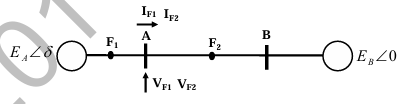
\includegraphics[width=0.8\textwidth]{figs/system_fault.png}
    \caption{Three-phase system with faults at $F_1$ and $F_2$.}
    \label{fig:system_fault}
\end{figure}

If the fault takes place at location $F_1$, the voltage and the current at bus $A$ are $V_{F1}$ and $I_{F1}$ respectively. If the fault takes place at location $F_2$, then the voltage and current at bus $A$ are $V_{F2}$ and $I_{F2}$ respectively. The correct statement about voltages and currents during faults at $F_1$ and $F_2$ is
\begin{enumerate}[label=(\Alph*)]
    \item $V_{F1}$ leads $I_{F1}$ and $V_{F2}$ leads $I_{F2}$
    \item $V_{F1}$ leads $I_{F1}$ and $V_{F2}$ lags $I_{F2}$
    \item $V_{F1}$ lags $I_{F1}$ and $V_{F2}$ leads $I_{F2}$
    \item $V_{F1}$ lags $I_{F1}$ and $V_{F2}$ lags $I_{F2}$
\end{enumerate}

\end{enumerate}

% Page ee_2014-2-_page-0009.jpg

\begin{enumerate}[label=Q\arabic*:, leftmargin=*, itemindent=0pt, start=16]

\item A 2-bus system and corresponding zero sequence network are shown in the figure.



The transformers $T_1$ and $T_2$ are connected as
\begin{enumerate}[label=(\Alph*)]
    \item $\text{YN}~\text{YN}$ and $\Delta$
    \item $\text{Y}_{\Delta}$ and $\Delta$
    \item $\text{Y}_{\Delta}$ and $\Delta~\text{YN}$
    \item $\Delta$ and $\text{Y}_{\Delta}$
\end{enumerate}

\item In the formation of Routh-Hurwitz array for a polynomial, all the elements of a row have zero values. This premature termination of the array indicates the presence of
\begin{enumerate}[label=(\Alph*)]
    \item only one root at the origin
    \item imaginary roots
    \item only positive real roots
    \item only negative real roots
\end{enumerate}

\item The root locus of a unity feedback system is shown below:
\begin{figure}[h]
    \centering
    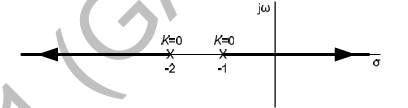
\includegraphics[width=0.8\textwidth]{figs/f1.png}
    \caption{Root locus plot for a unity feedback system.}
    \label{fig:root_locus}
\end{figure}

The closed loop transfer function of the system is
\begin{enumerate}[label=(\Alph*)]
    \item $\dfrac{C(s)}{R(s)} = \dfrac{K}{(s+1)(s+2)}$
    \item $\dfrac{C(s)}{R(s)} = \dfrac{-K}{(s+1)(s+2)+K}$
    \item $\dfrac{C(s)}{R(s)} = \dfrac{K}{(s+1)(s+2) - K}$
    \item $\dfrac{C(s)}{R(s)} = \dfrac{K}{(s+1)(s+2) + K}$
\end{enumerate}

\item Power consumed by a balanced three-phase, three-wire load is measured by the two wattmeter method. The first wattmeter reads twice that of the second. The load impedance angle in radians is
\begin{enumerate}[label=(\Alph*)]
    \item $\pi/12$
    \item $\pi/8$
    \item $\pi/6$
    \item $\pi/3$
\end{enumerate}

\item In an oscilloscope screen, linear sweep is applied at the
\begin{enumerate}[label=(\Alph*)]
    \item vertical axis
    \item horizontal axis
    \item origin
    \item both horizontal and vertical axis
\end{enumerate}

\end{enumerate}



% Page ee_2014-2-_page-0013.jpg
\begin{enumerate}[label=Q\arabic*:, leftmargin=*, itemindent=0pt, start=31]

\item In an unbalanced three phase system, phase current $I_a = 1\angle(-90^\circ)$ pu, negative sequence current $I_{b2} = 4\angle(-150^\circ)$ pu, zero sequence current $I_{c0} = 3\angle90^\circ$ pu. The magnitude of phase current $I_b$ in pu is
\begin{enumerate}[label=(\Alph*)]
    \item 1.00
    \item 7.81
    \item 11.53
    \item 13.00
\end{enumerate}

\item The following four vector fields are given in Cartesian coordinates. The vector field which does not satisfy the property of magnetic flux density is
\begin{enumerate}[label=(\Alph*)]
    \item $y^2 \mathbf{a}_x + z^2 \mathbf{a}_y + x^2 \mathbf{a}_z$
    \item $z^2 \mathbf{a}_x + x^2 \mathbf{a}_y + y^2 \mathbf{a}_z$
    \item $x^2 \mathbf{a}_x + y^2 \mathbf{a}_y + z^2 \mathbf{a}_z$
    \item $y^2 z^2 \mathbf{a}_x + x^2 z^2 \mathbf{a}_y + x^2 y^2 \mathbf{a}_z$
\end{enumerate}

\item The function shown in the figure can be represented as
\[
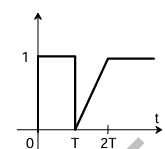
\includegraphics[width=0.45\textwidth]{figs/f2.png}
\]
\begin{enumerate}[label=(\Alph*)]
    \item $u(t) - u(t-T) + \frac{t-T}{T} u(t-T) - \frac{t-2T}{T} u(t-2T)$
    \item $u(t) + \frac{t}{T} u(t-T) - \frac{t}{T} u(t-2T)$
    \item $u(t) - u(t-T) + \frac{t-T}{T} u(t-T) - \frac{t-2T}{T} u(t)$
    \item $u(t) + \frac{t-T}{T} u(t-T) - \frac{t-2T}{T} u(t-2T)$
\end{enumerate}

\item Let $X(z) = \frac{1}{1-z^{-3}}$ be the Z-transform of a causal signal $x[n]$. Then, the values of $x[2]$ and $x[3]$ are
\begin{enumerate}[label=(\Alph*)]
    \item 0 and 0
    \item 0 and 1
    \item 1 and 0
    \item 1 and 1
\end{enumerate}

\item Let $f(t)$ be a continuous time signal and let $F(\omega)$ be its Fourier transform defined by
\[
F(\omega) = \int_{-\infty}^{\infty} f(t) e^{-j \omega t} dt
\]
Define $g(t)$ by
\[
g(t) = \int_{-\infty}^{\infty} F(u) e^{-j u t} du
\]
What is the relationship between $f(t)$ and $g(t)$?
\begin{enumerate}[label=(\Alph*)]
    \item $g(t)$ would always be proportional to $f(t)$
    \item $g(t)$ would be proportional to $f(t)$ if $f(t)$ is even
    \item $g(t)$ would be proportional to $f(t)$ only if $f(t)$ is sinusoidal
    \item $g(t)$ would never be proportional to $f(t)$
\end{enumerate}

\end{enumerate}
%--------------------------

% Page ee_2014-2-_page-0014.jpg
\begin{enumerate}[label=Q\arabic*:, leftmargin=*, itemindent=0pt, start=25]

\item Figure shows four electronic switches (i)-(iv). Which can block voltages of either polarity (applied between terminals 'a' and 'b') when the active device is OFF?
\[
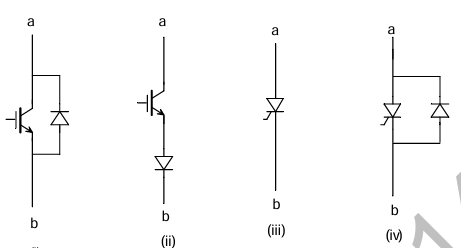
\includegraphics[width=0.8\textwidth]{figs/f3.png}
\]
\begin{enumerate}[label=(\Alph*)]
    \item (i), (ii) and (iii)
    \item (ii), (iii) and (iv)
    \item (ii) and (iii)
    \item (i) and (iv)
\end{enumerate}

\end{enumerate}

% Page ee_2014-2-_page-0015.jpg
\begin{enumerate}[label=Q\arabic*:, leftmargin=*, itemindent=0pt, start=26]

\item Let $g: [0, \infty) \to [0, \infty)$, $g(x) = x - [x]$, where $[x]$ is the greatest integer less than or equal to $x$. The value of the constant term in the Fourier series expansion for $g(x)$ is \rule{3cm}{0.15mm}.

\item A fair coin is tossed $n$ times. The probability that the difference between the number of heads and tails is $(n-3)$ is
\begin{enumerate}[label=(\Alph*)]
    \item $2^{-n}$
    \item 0
    \item ${ n \choose (n-3)/2 } 2^{-n}$
    \item $2^{-(n+3)}$
\end{enumerate}

\item The line integral of $F = y z \mathbf{i}$ in the counterclockwise direction, along the circle $x^2 + y^2 = 1$, at $z=1$ is
\begin{enumerate}[label=(\Alph*)]
    \item $-2\pi$
    \item $-\pi$
    \item $\pi$
    \item $2\pi$
\end{enumerate}

\item An incandescent lamp is marked 40 W, 240 V. If resistance at room temperature (26$^\circ$C) is 120 $\Omega$ and temperature coefficient of resistance is $4.5 \times 10^{-3}/\ ^\circ$C, then its 'ON' state filament temperature $^\circ$C is approximately \rule{4cm}{0.15mm}.

\item In the figure, the value of resistor $R$ is $(25 + I/2)$ ohms, where $I$ is the current in amperes. The current $I$ is
\[
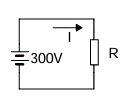
\includegraphics[width=0.3\textwidth]{figs/f4.png}
\]

\end{enumerate}

% Page ee_2014-2-_page-0016.jpg
\begin{enumerate}[label=Q\arabic*:, leftmargin=*, itemindent=0pt, start=40]

\item A distribution feeder of 1 km length having resistance but negligible reactance is fed from both ends by 400 V, 50 Hz balanced sources. Both sources $S_1$, $S_2$ are in phase. The feeder supplies concentrated loads of unity power factor as shown in figure.
\[
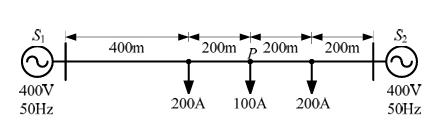
\includegraphics[width=0.9\textwidth]{figs/f5.png}
\]
The contributions of $S_1$ and $S_2$ in 100 A current supplied at location $P$ respectively, are
\begin{enumerate}[label=(\Alph*)]
    \item 75 A and 25 A
    \item 50 A and 50 A
    \item 25 A and 75 A
    \item 0 A and 100 A
\end{enumerate}

\item A two bus power system shown in the figure supplies load of $1.0 + j0.5$ p.u.
\[
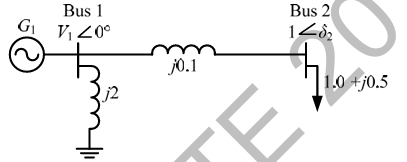
\includegraphics[width=0.7\textwidth]{figs/f6.png}
\]
The values of $V_1$ in p.u. and $\delta_2$ respectively are
\begin{enumerate}[label=(\Alph*)]
    \item 0.95 and $6.00^\circ$
    \item 1.05 and $-5.44^\circ$
    \item 1.1 and $-6.00^\circ$
    \item 1.1 and $-27.12^\circ$
\end{enumerate}

\item The fuel cost functions of two power plants are:
Plant $P_1 : C_1 = 0.05 {P_{g1}}^2 + A P_{g1} + B$ \\
Plant $P_2 : C_2 = 0.10 {P_{g2}}^2 + 3A P_{g2} + 2B$ \\
If the two plants optimally share 1000 MW load at incremental fuel cost of 100 Rs/MWh, the ratio of load shared by $P_1$ and $P_2$ is:
\begin{enumerate}[label=(\Alph*)]
    \item 1:4
    \item 2:3
    \item 3:2
    \item 4:1
\end{enumerate}

\item The overcurrent relays for the line protection and loads connected at buses are shown.
\[
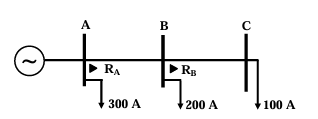
\includegraphics[width=0.7\textwidth]{figs/f7.png}
\]
The relays are IDMT in nature with characteristic:
\[
t_{op} = \frac{0.14 \times \text{TimeMultiplierSetting}}{(\text{PlugSettingMultiplier})^{0.02} - 1}
\]
The maximum and minimum fault currents at bus B are 2000 A and 500 A. Assuming the time multiplier setting and plug setting for relay $R_B$ to be 0.1 and 5A respectively, the operating time of $R_B$ (in seconds) is \rule{3cm}{0.15mm}.

\end{enumerate}

% Page ee_2014-2-_page-0014.jpg
\begin{enumerate}[label=Q\arabic*:, leftmargin=*, itemindent=0pt, start=36]

\item The core loss of a single phase, 230/115 V, 50 Hz power transformer is measured from 230 V side by feeding the primary (230 V side) from a variable voltage–variable frequency source while keeping the secondary open circuited. The core loss is measured to be 1050 W for 230 V, 50 Hz input, and again 500 W for 138 V, 30 Hz input. The hysteresis and eddy current losses at 230 V, 50 Hz input are:
\begin{enumerate}[label=(\Alph*)]
    \item 508 W and 542 W
    \item 468 W and 582 W
    \item 498 W and 552 W
    \item 488 W and 562 W
\end{enumerate}

\item A 15 kW, 230 V dc shunt motor has armature resistance 0.4 $\Omega$ and field resistance 230 $\Omega$. At no load and rated voltage, the motor runs at 1400 rpm, and the line current is 5 A. At full load, it draws 70 A. Neglect armature reaction. The full load speed of the motor, in rpm: \rule{3cm}{0.15mm}

\item A 3-phase, 50 Hz, six pole induction motor has rotor resistance 0.1 $\Omega$ and reactance 0.92 $\Omega$. Neglect stator voltage drop and assume constant rotor resistance. For full load slip 3\%, the ratio of maximum torque to full load torque is:
\begin{enumerate}[label=(\Alph*)]
    \item 1.567
    \item 1.712
    \item 1.948
    \item 2.134
\end{enumerate}

\item A three-phase synchronous generator is to be connected to the infinite bus. The lamps are connected for synchronization as shown (figure). The phase sequence of bus voltage is R-Y-B and that of incoming generator voltage is R'-Y'-B'. It was found that the lamps darken in sequence $L_a$-$L_b$-$L_c$. The phase sequence of incoming generator is:
\begin{enumerate}[label=(\Alph*)]
    \item opposite to infinite bus and its frequency is more than infinite bus
    \item opposite to infinite bus but its frequency is less than infinite bus
    \item same as infinite bus and its frequency is more than infinite bus
    \item same as infinite bus and its frequency is less than infinite bus
\end{enumerate}

\end{enumerate}

\end{document}


\end{document}

\end{document}


%\documentclass{article}
% \usepackage{graphicx} % Required for inserting images

% \title{Gate 2 prime}
% \author{Bob The Robber}
% \date{August 2025}

% \begin{document}

% \maketitle

% \section{Introduction}

% \end{document}
